\documentclass[12pt]{article}
\usepackage{graphicx,float}
\usepackage{listings}
\usepackage{xcolor}
\usepackage{circuitikz}

\definecolor{codegreen}{rgb}{0,0.6,0}
\definecolor{codegray}{rgb}{0.5,0.5,0.5}
\definecolor{codepurple}{rgb}{0.58,0,0.82}
\definecolor{backcolour}{rgb}{0.95,0.95,0.92}


\lstdefinelanguage{SPICE}{
  keywords={tran,ac,dc,subckt,meas,plot,print,control,run,end,endc, hardcopy},
  morecomment=[l]{*},
  morecomment=[l]{\$},
  morecomment=[s]{/*}{*/},
  morestring=[b]',
  morestring=[b]",
  ndkeywords={r,r1,r2,r3,r4,r5,l,l1,l2,l3,l4,l5,c,c1,c2,c3,c4,c5,v,vin,m,m1,m2,m3,m4,m5,d,d1,d2,d3,d4,d5,vdb, pulse,sin,i,pwl,exp},
  keywordstyle=\color{blue}\bfseries,
  ndkeywordstyle=\color{codegreen}\bfseries,
  identifierstyle=\color{black},
  commentstyle=\color{purple}\ttfamily,
  stringstyle=\color{red}\ttfamily,
  sensitive=true
}

\lstdefinestyle{mystyle}{
	backgroundcolor=\color{backcolour},   
    commentstyle=\color{codegreen},
    keywordstyle=\color{magenta},
    numberstyle=\tiny\color{codegray},
    stringstyle=\color{codepurple},
    basicstyle=\ttfamily\footnotesize,
    breakatwhitespace=false,         
    breaklines=true,                 
    captionpos=b,                    
    keepspaces=true,                 
    numbers=left,                    
    numbersep=5pt,                  
    showspaces=false,                
    showstringspaces=false,
    showtabs=false,                  
    tabsize=4
}

\lstset{style=mystyle}


% Title[Enter title of the experiment here]
\title{EE230: Lab-2\\
Unregulated DC Power Supply Learning}

% Author[Enter details of author here]
\author{Prateek Garg, 20D070060}

% begin the document.
\begin{document}
\noindent
% make a title page.[this creates title page]
\maketitle

\section{Overview of the experiment} %[This segment creates Section as seen in document]

\subsection{Aim of the experiment}%[This segment creates sebsections under the same section]
\begin{enumerate}
  \item Understanding the limits of performance of a Zener regulator
  \item Understanding a BJT based series voltage regulator to appreciate the basic blocks of an IC
  voltage regulator.
\end{enumerate}
\subsection{Methods}
We start by analysing the circuits and then simulating in ngspice to check against theoretical expectations.  
\section{Design}
%Add circuit Diagrams here
%With accompaying Explanantions 
\subsection{Zener Regulator}
\begin{figure}[H]
  \begin{center}
    \makebox{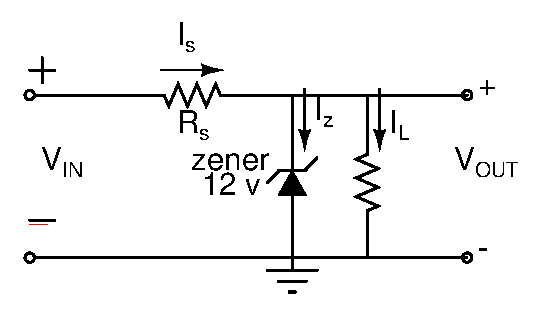
\includegraphics{zener.eps}}
\end{center}
\end{figure}

\textbf{In non conduction region : }
$$I_{z} = 0$$
$$V_{out} < 12V$$
$$V_{out}=\frac{V_{in}}{R_s+R_l}$$

\textbf{In conduction region : }
Using $R_{z}=125\Omega$ and $V_{z}$=12V
$$V_{out} \ge 12V$$
$$V_{out} = (V_{in}/R_s+12/125)/(1/R_s+1/R_z+1/R_l)$$
$$I_s=(V_{in}-V_{out})/R_s$$
$$I_z=(V_{out}-12)/125$$

\subsection{BJT Series Regulator}
\begin{figure}[H]
  \begin{center}
    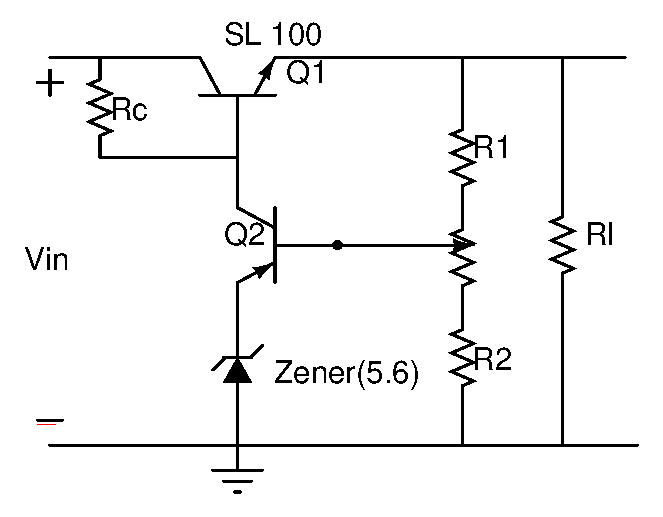
\includegraphics{BJT.eps}
\end{center}
\end{figure}

\newpage
\section{Simulation results}

\subsection{Zener Regulator}
\subsubsection{Code snippet}
\lstinputlisting[language=SPICE]{../Zener-Regulator-A.cir}
\subsubsection{Simulation results}
%\makebox[\textwidth]{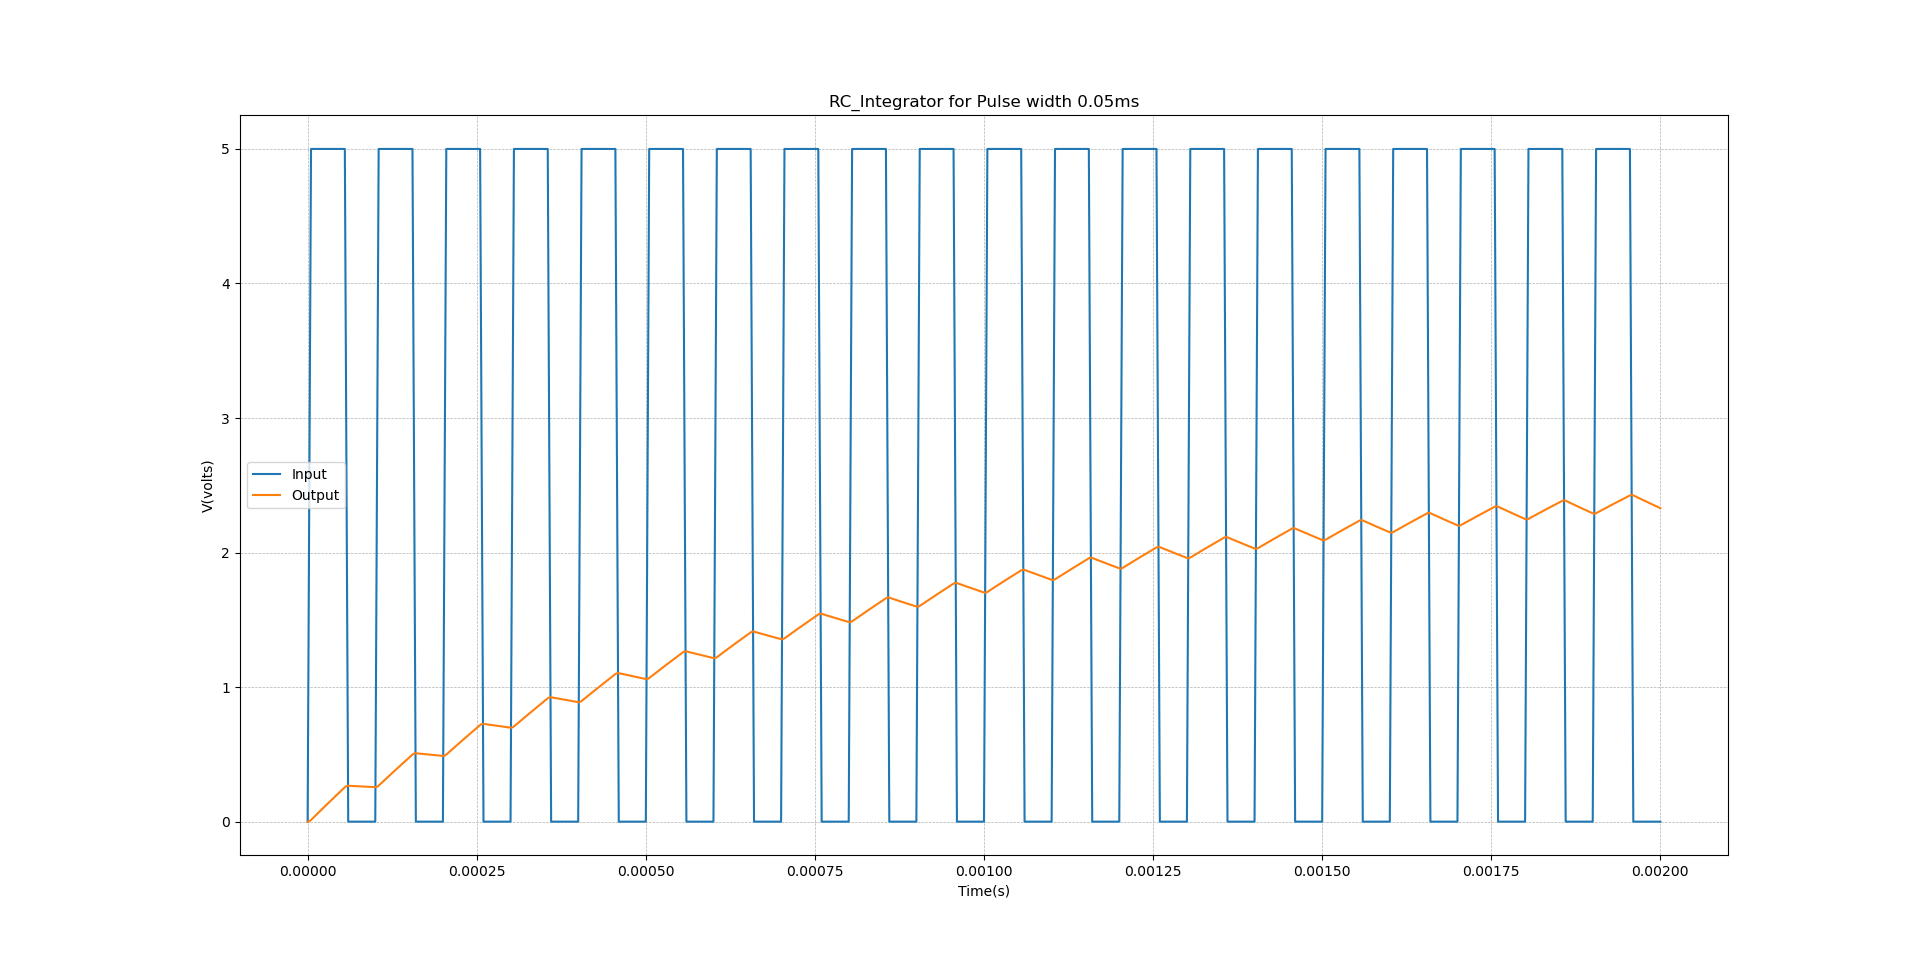
\includegraphics[width=\paperwidth]{RC_Integrator_6.png}}

\subsection{BJT Series Regulator}
\subsubsection{Code snippet}
\lstinputlisting[language=SPICE]{../BJT-Regulator-A.cir}
\subsubsection{Simulation results}
\textbf{\large Zener Regulator}
\begin{figure}[H]
  \begin{center}
    \makebox[0.8\textwidth]{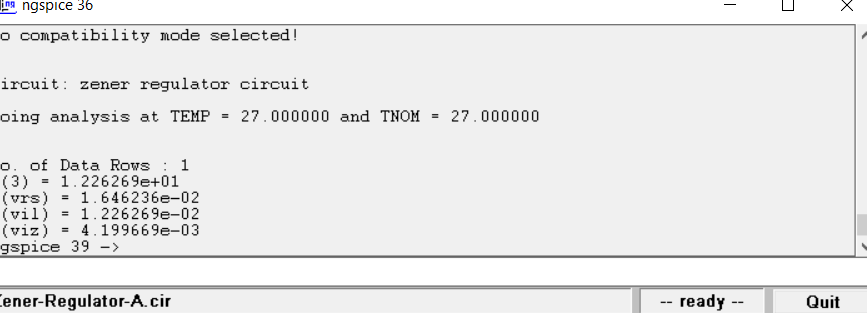
\includegraphics[width=0.8\paperwidth]{Zener-Regulator-A.png}}
\end{center}
\end{figure}
\begin{figure}[H]
  \begin{center}
    \makebox[0.8\textwidth]{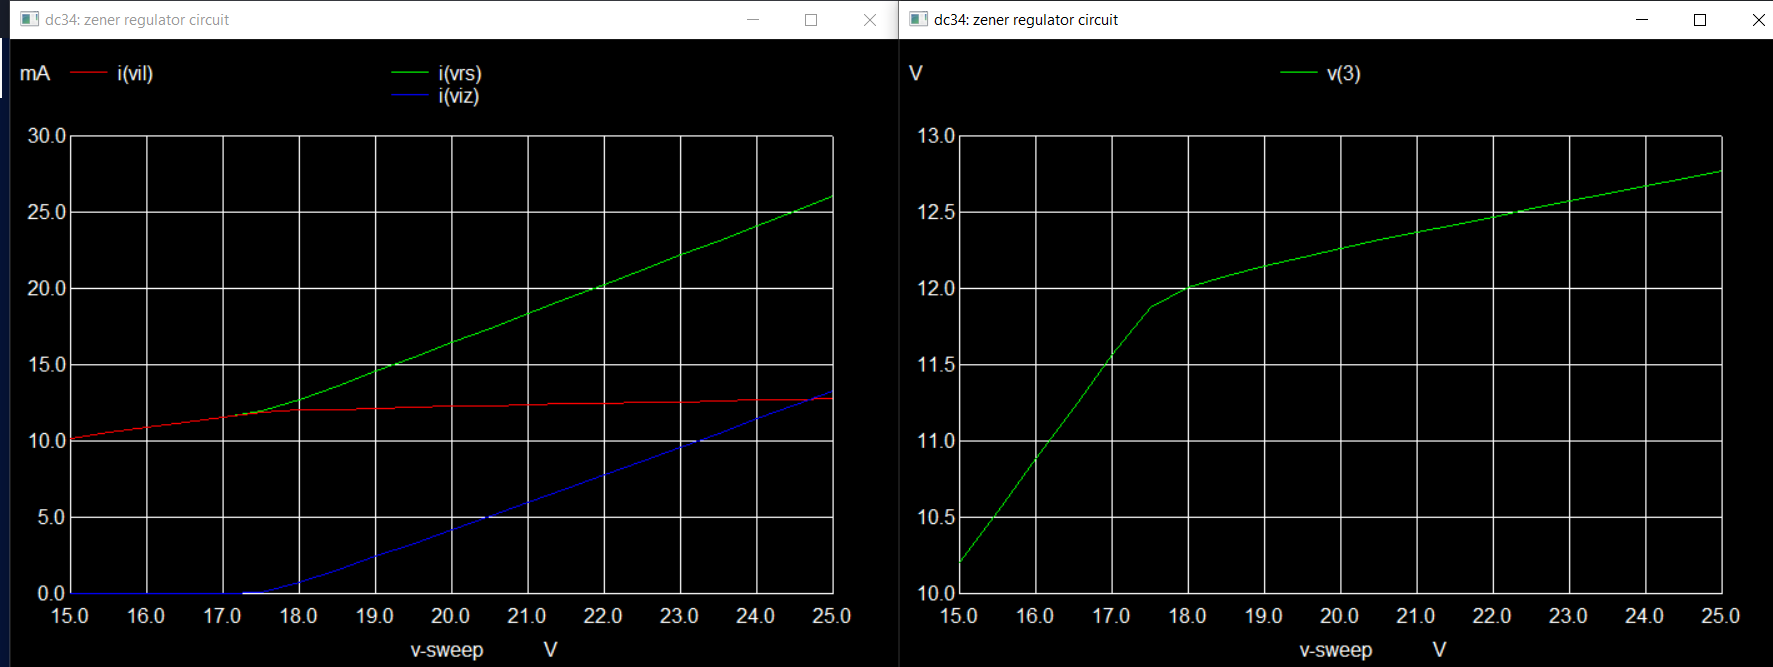
\includegraphics[width=0.8\paperwidth]{Zener-Regulator-B.png}}
\end{center}
\end{figure}
\begin{figure}[H]
  \begin{center}
    \makebox[0.8\textwidth]{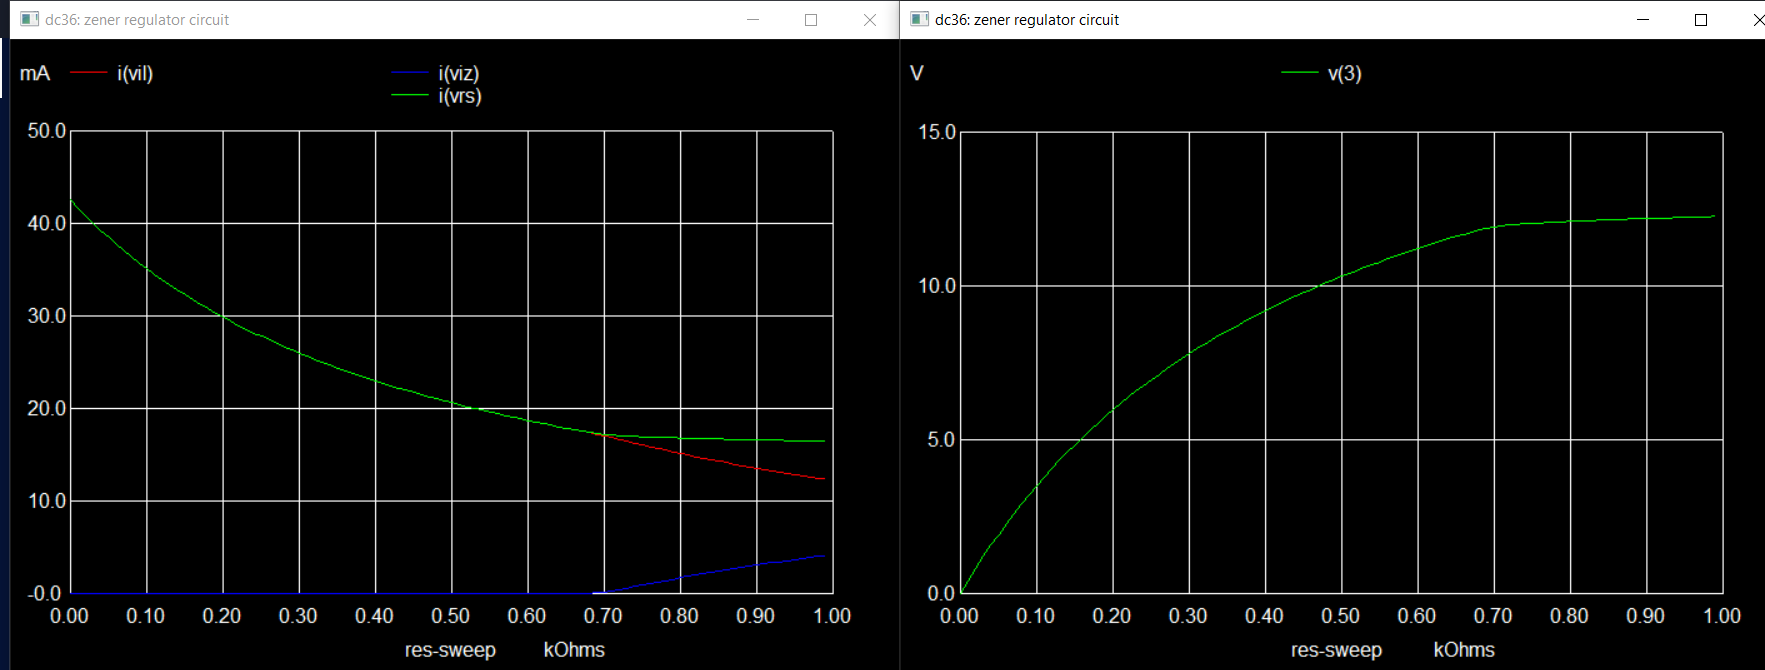
\includegraphics[width=0.8\paperwidth]{Zener-Regulator-C.png}}
\end{center}
\end{figure}

\textbf{\large BJT Series Regulator}
\begin{figure}[H]
  \begin{center}
    \makebox[0.8\textwidth]{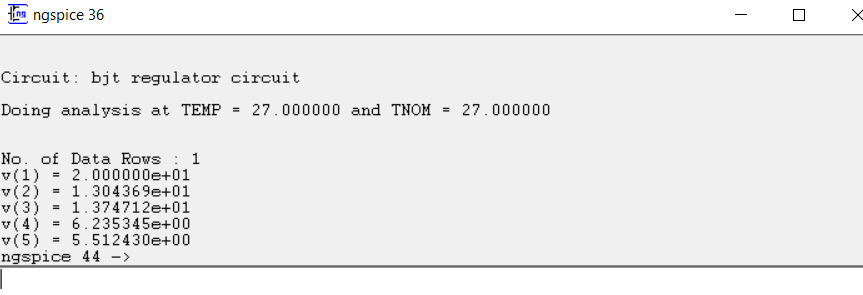
\includegraphics[width=0.8\paperwidth]{BJT-Regulator-A.png}}
\end{center}
\end{figure}
\begin{figure}[H]
  \begin{center}
    \makebox[0.8\textwidth]{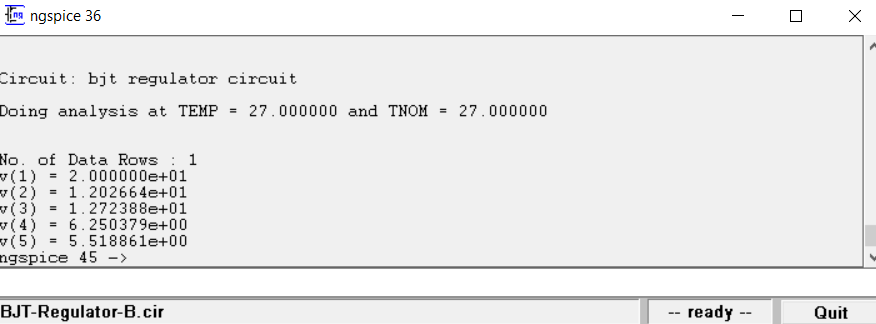
\includegraphics[width=0.8\paperwidth]{BJT-Regulator-B.png}}
\end{center}
\end{figure}
\begin{figure}[H]
  \begin{center}
    \makebox[0.8\textwidth]{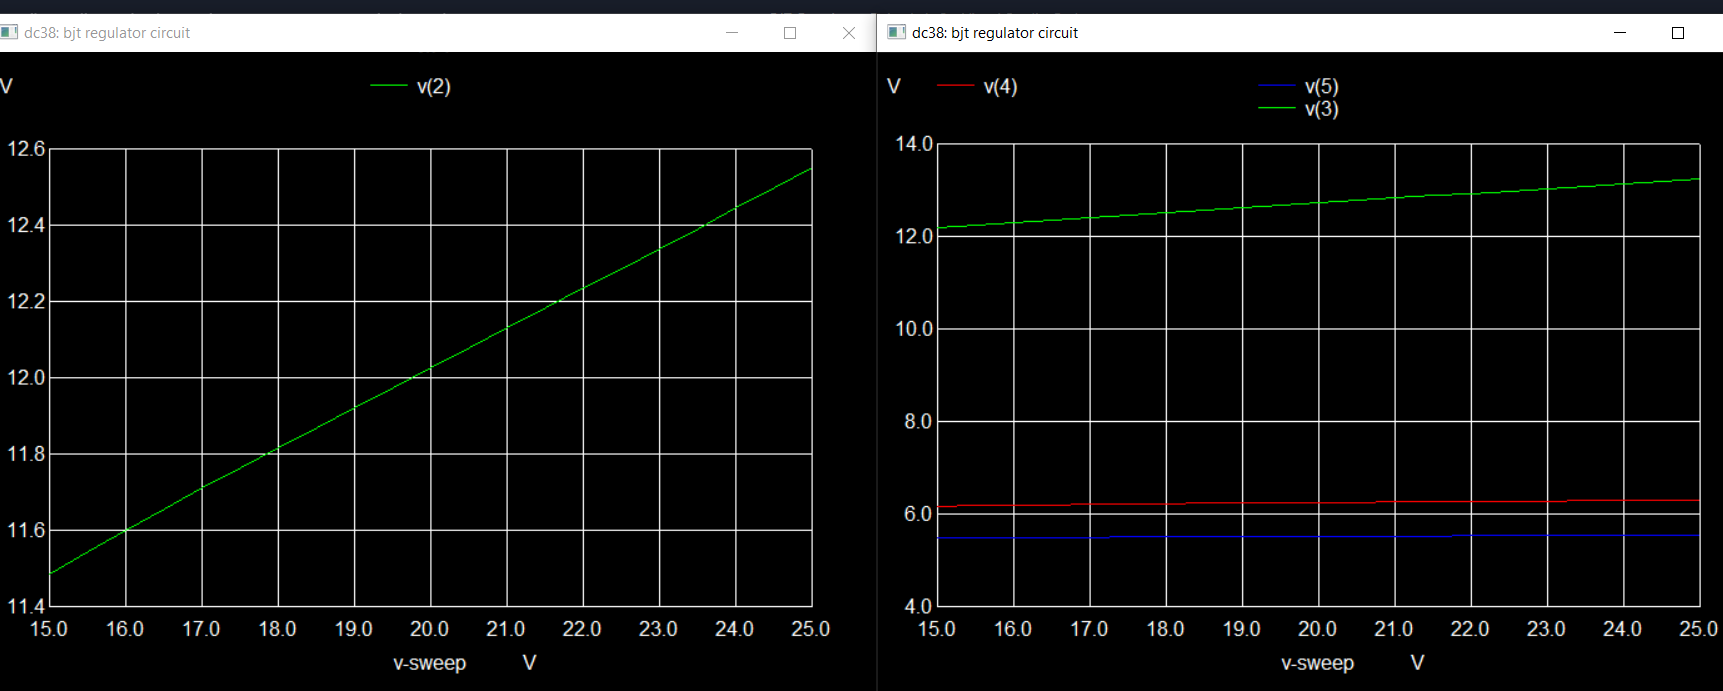
\includegraphics[width=0.8\paperwidth]{BJT-Regulator-C.png}}
\end{center}
\end{figure}


\section{Experiment completion status}
All the sections were completed
\end{document}
